\documentclass{beamer}
%
% Choose how your presentation looks.
%
% For more themes, color themes and font themes, see:
% http://deic.uab.es/~iblanes/beamer_gallery/index_by_theme.html
%
\mode<presentation>
{
  \usetheme{Madrid}      % or try Darmstadt, Madrid, Warsaw, ...
  \usecolortheme{beaver} % or try albatross, beaver, crane, ...
  \usefonttheme{serif}  % or try serif, structurebold, ...
  \setbeamertemplate{navigation symbols}{}
  \setbeamertemplate{caption}[numbered]
} 

\usepackage[english]{babel}

\usepackage[utf8x]{inputenc}
\usepackage{xcolor}
\usepackage{listings}
\usepackage{textpos}


% addional configuration from sam
\usepackage{bibgerm}
\usepackage{hyperref}
\usepackage{cite}
\usepackage{etoolbox}
\usepackage{listings}
\usepackage{float}%
\usepackage{verbatim}
\usepackage{filecontents}
\usepackage{siunitx}
\sisetup{per=slash, load=abbr}
\usepackage{tikz}
\usepackage{pgfplots}
\pgfplotsset{width=7cm,compat=newest}
\usepackage[autostyle=true,german=quotes]{csquotes}
\usepackage{multirow}
\usepackage{hhline}
\usepackage{amsmath}
\RequirePackage{helvet}
\renewcommand{\familydefault}{\sfdefault}





\lstset
{
    language=[LaTeX]TeX,
    breaklines=true,
    basicstyle=\tt\scriptsize,
    %commentstyle=\color{green}
    keywordstyle=\color{blue},
    %stringstyle=\color{black}
    identifierstyle=\color{magenta},
}

\renewcommand{\rmdefault}{phv} % Arial
\renewcommand{\sfdefault}{phv} % Arial

\setbeamertemplate{frametitle}[default][center]

\addtobeamertemplate{frametitle}{}{%
\begin{textblock*}{100mm}(.88\textwidth,-.87cm)

\includegraphics[height=0.8cm,width=1.3cm]{ffhslogo}
\end{textblock*}}


\addtobeamertemplate{frametitle}{}{%
\begin{textblock*}{100mm}(-.02\textwidth,-.9cm)
%
\includegraphics[height=1.5cm,width=1.5cm]{chip}
\end{textblock*}}


\title[Durch effizientere Software Energie sparen]{Durch effizientere Software Energie sparen \newline \newline Analyse des Energieverbrauchs pro Befehlssatz eines Prozessors}
\author{Samuel Riolo}
\institute{Bachelor Thesis \textendash FFHS}
\date{5. September 2016}


\begin{document}
% https://github.com/zemirco/tu-darmstadt-latex-thesis


% Farbpalette A
\definecolor{blau_1a}{RGB}{93,133,195}
\definecolor{blau_2a}{RGB}{0,156,218}
\definecolor{gruen_3a}{RGB}{80,182,149}
\definecolor{gruen_4a}{RGB}{175,204,80}
\definecolor{gruen_5a}{RGB}{221,223,72}
\definecolor{orange_6a}{RGB}{255,224,92}
\definecolor{orange_7a}{RGB}{248,186,60}
\definecolor{rot_8a}{RGB}{238,122,52}
\definecolor{rot_9a}{RGB}{233,80,62}
\definecolor{lila_10a}{RGB}{201,48,142}
\definecolor{lila_11a}{RGB}{128,69,151}

% Farbpalette B
\definecolor{blau_1b}{RGB}{0,90,169}
\definecolor{blau_2b}{RGB}{0,131,204}
\definecolor{gruen_3b}{RGB}{0,157,129}
\definecolor{gruen_4b}{RGB}{153,192,0}
\definecolor{gruen_5b}{RGB}{201,212,0}
\definecolor{orange_6b}{RGB}{253,202,0}
\definecolor{orange_7b}{RGB}{245,163,0}
\definecolor{rot_8b}{RGB}{236,101,0}
\definecolor{rot_9b}{RGB}{230,0,26}
\definecolor{lila_10b}{RGB}{166,0,132}
\definecolor{lila_11b}{RGB}{114,16,133}




\begin{frame}
  \titlepage
\end{frame}

% Uncomment these lines for an automatically generated outline.
\begin{frame}{Outline}
\frametitle{Inhaltsverzeichnis}
    \tableofcontents[]
\end{frame}



\section{Um was geht es -- in K{\"u}rze} 
\begin{frame}
\frametitle{Um was geht es -- in K{\"u}rze} 
\begin{itemize}
\item Energieverbrauch pro Befehlssatz
\item Erstellung eines Benchmarks
\item Befehlssatz x-mal ausführen und Strom messen
\end{itemize}


\begin{figure}[!htb]\centering
   \begin{minipage}{0.49\textwidth}
    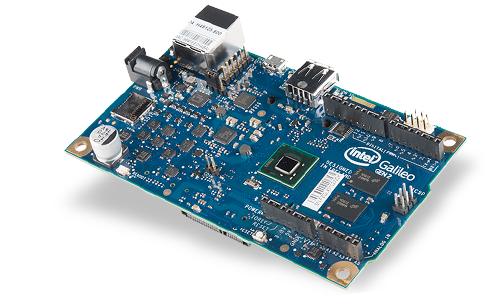
\includegraphics[height=100px]{iot_galileo.png}
   \end{minipage}
   \begin {minipage}{0.49\textwidth}
     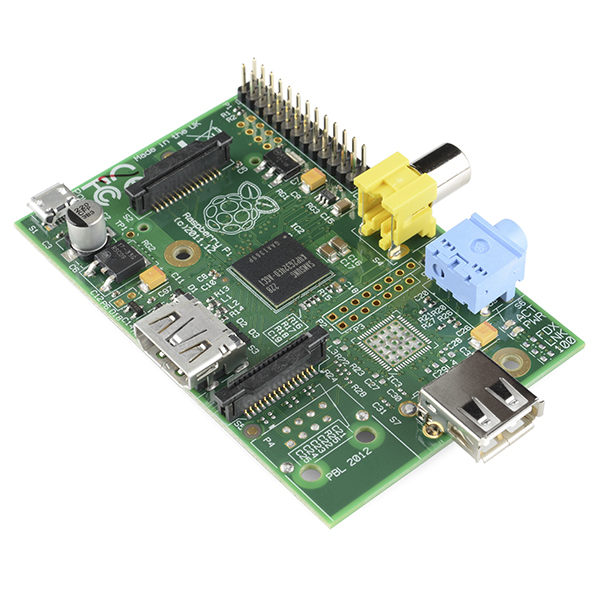
\includegraphics[height=100px]{raspberry-pi-2.png}
   \end{minipage}
\end{figure}
\end{frame}


\section{Resultate} 

\begin{frame}
\frametitle{Resultate Raspberry PI (ARM)}
\begin{figure}[H]
\centering
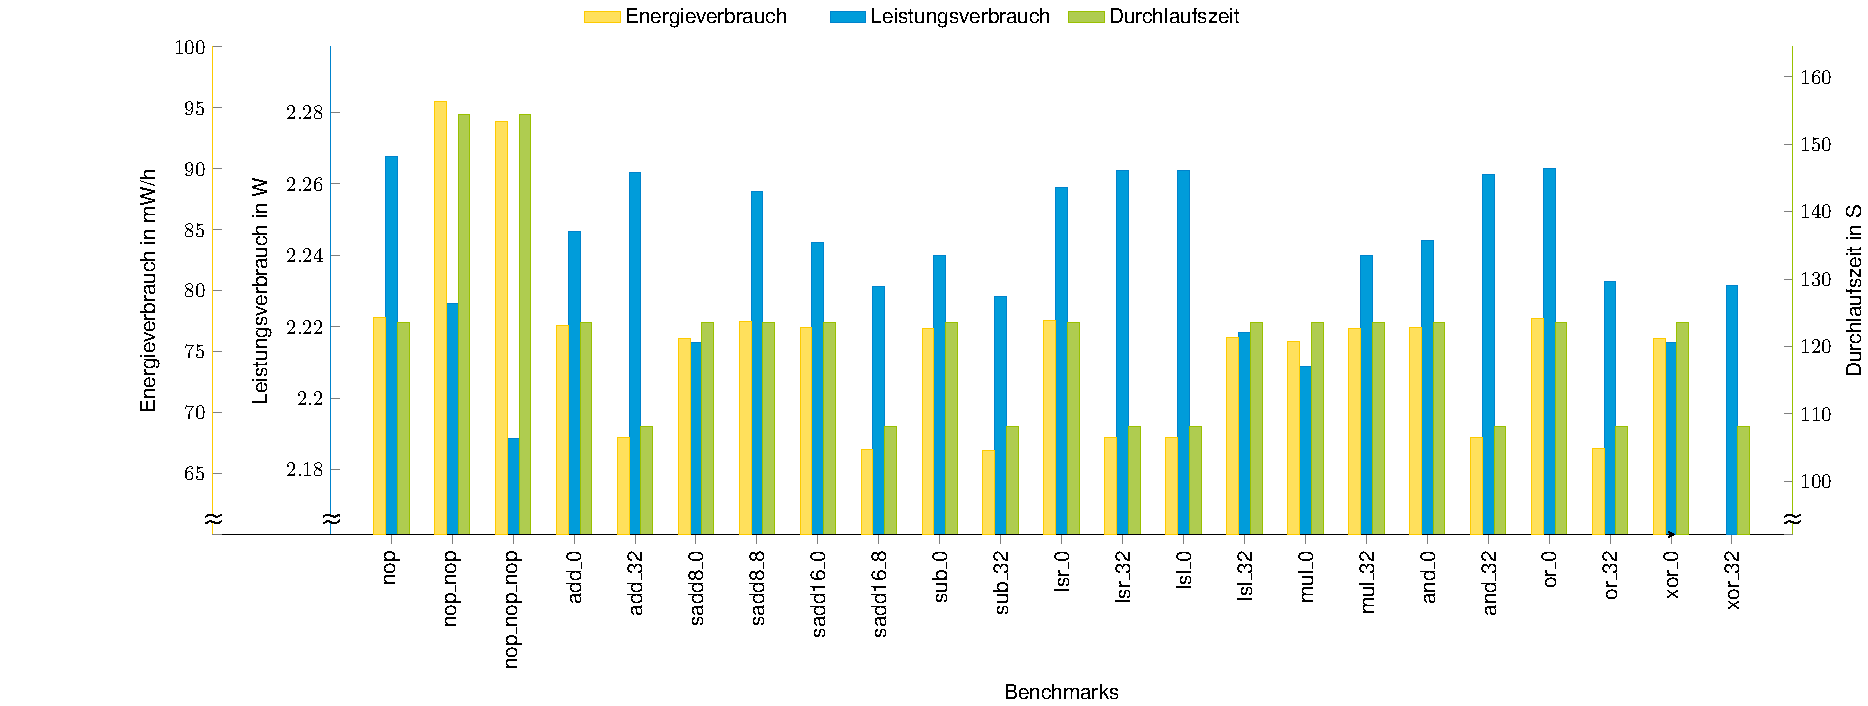
\includegraphics[width=1\textwidth]{raspberry_results.pdf}
\end{figure}
\end{frame}

\begin{frame}
\frametitle{Resultate Galileo (x86)}
\begin{figure}[H]
\centering
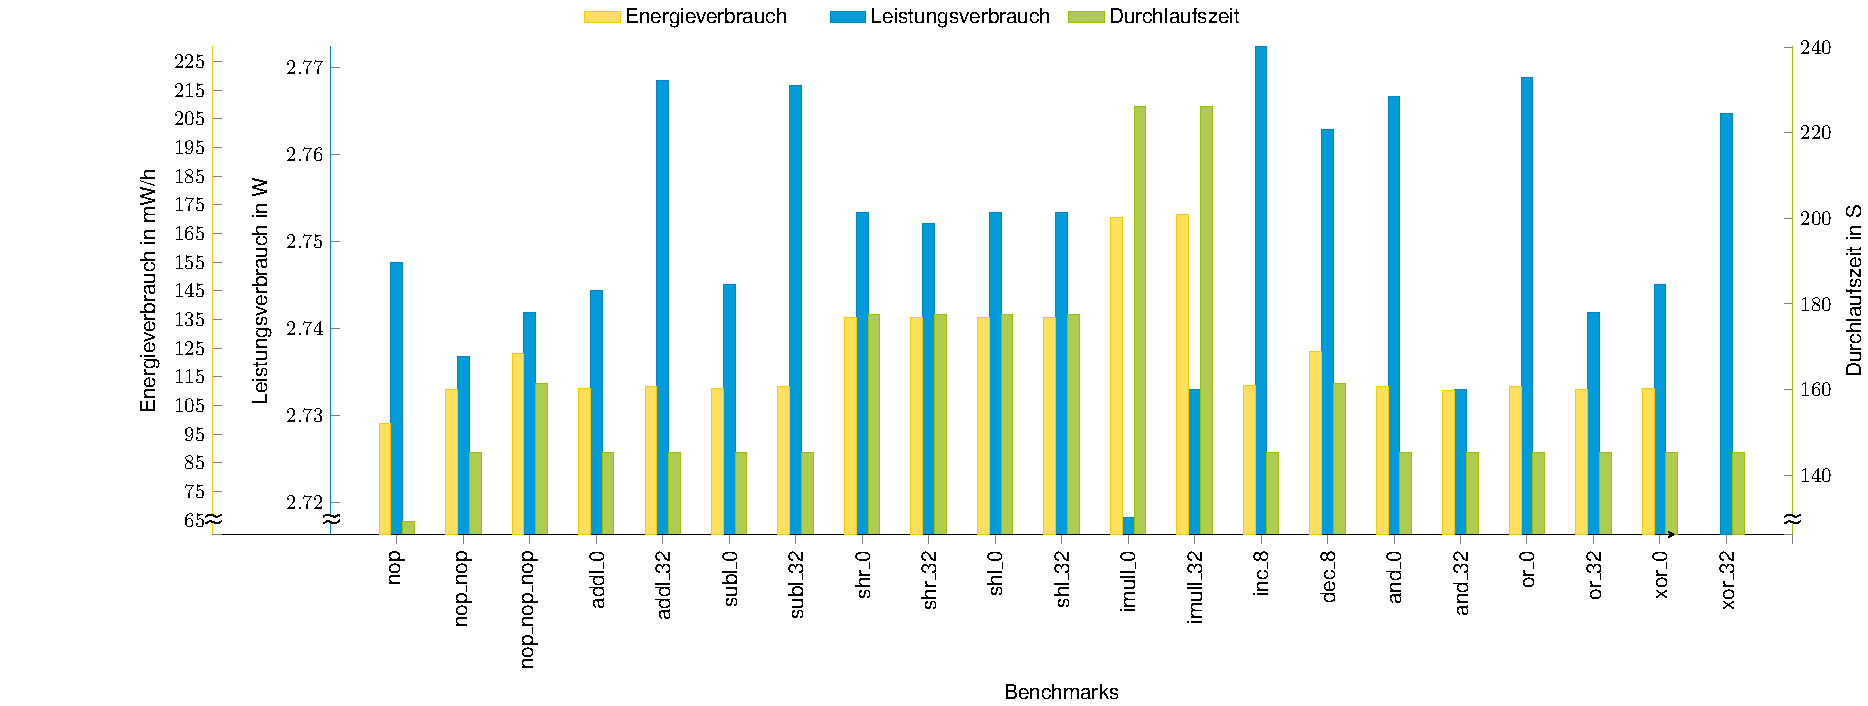
\includegraphics[width=1\textwidth]{galileo_results.pdf}
\end{figure}
\end{frame}

\section{Abbildungen} 
\begin{frame}
\frametitle{Benchmark}
\begin{figure}[H]
\centering
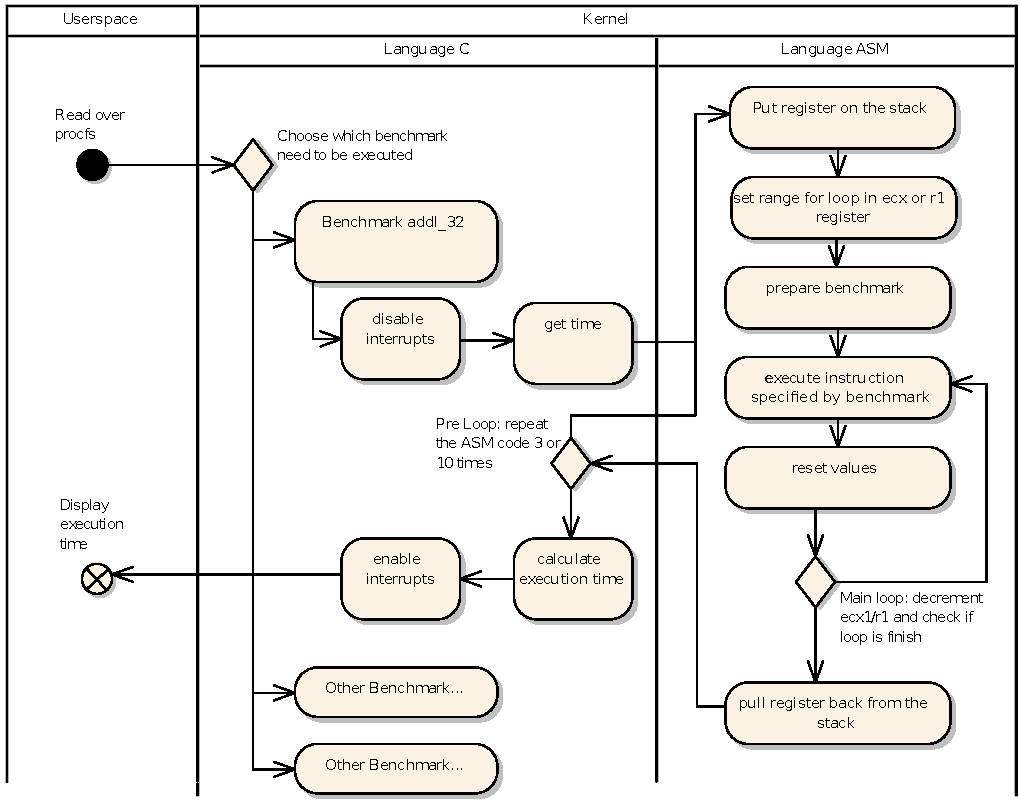
\includegraphics[width=0.8\textwidth]{../thesis/images/benchmark_ea.pdf}
\end{figure}
\end{frame}



\begin{frame}
\frametitle{Programm Struktur}
\begin{figure}[H]
\centering
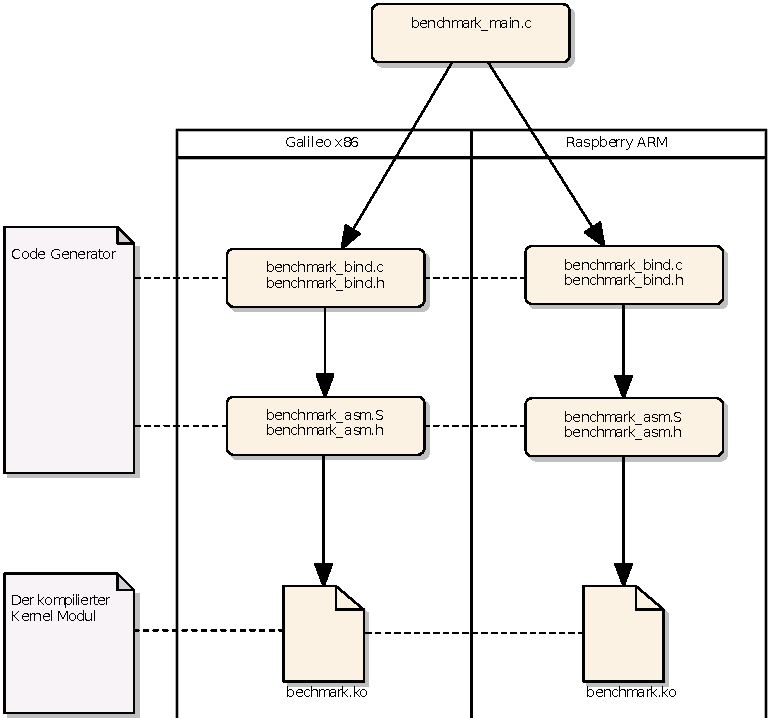
\includegraphics[width=0.65\textwidth]{../thesis/images/filestructure.pdf}
\end{figure}
\end{frame}

\begin{frame}
\frametitle{Interrupts}
\begin{figure}[H]
\centering
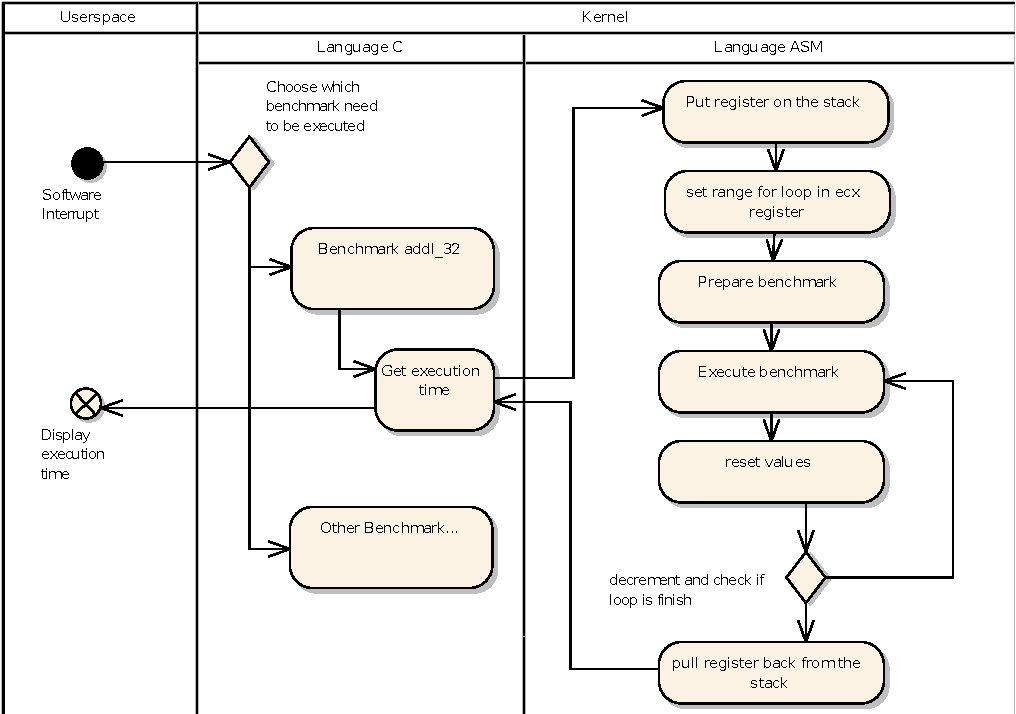
\includegraphics[width=0.65\textwidth]{../thesis/images/interrupt_ea.pdf}
\end{figure}
\end{frame}


\begin{frame}
\frametitle{Aufbau eins Prozessor}
\begin{figure}[H]
\centering
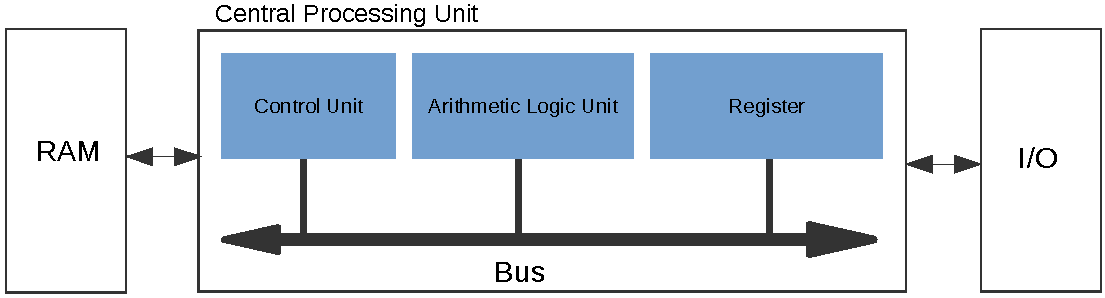
\includegraphics[width=0.8\textwidth]{../thesis/images/cpu.pdf}
\end{figure}
\end{frame}


\begin{frame}
\frametitle{Kernel des Linux Betriebssystem}
\begin{figure}[H]
\centering
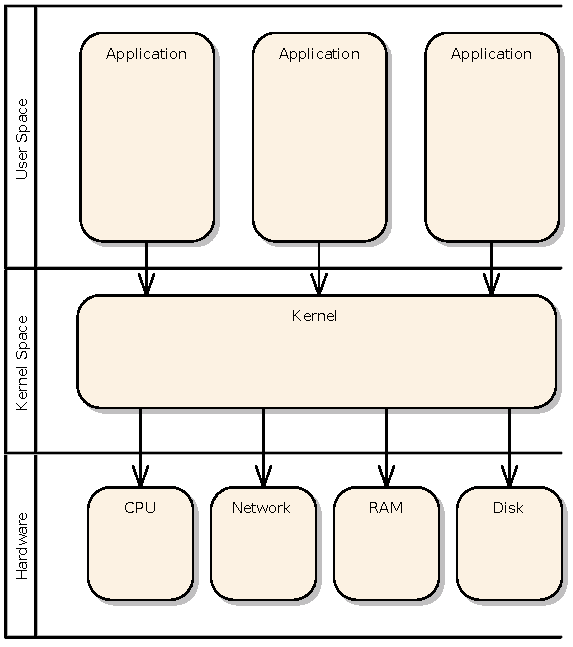
\includegraphics[width=0.5\textwidth]{../thesis/images/kernel.pdf}
\end{figure}
\end{frame}



\section{Code Snippet} 
\begin{frame}[fragile]
\frametitle{C} 

\lstset{language=C,
                basicstyle=\ttfamily\small,
                keywordstyle=\color{blue}\ttfamily,
                stringstyle=\color{red}\ttfamily,
                commentstyle=\color{green}\ttfamily,
                morecomment=[l][\color{magenta}]{\#}
}
\begin{lstlisting}
int benchmark_show_addl_32(struct seq_file* m, void* v)
{
    int i;
    unsigned long flags;
    struct timeval start_time;
    unsigned long  exec_time;

    local_irq_save(flags);
    start_time = timer_start();
    for (i = 0; i < REPEAT_BENCHMARK; i++)
        benchmark_addl_32();
    exec_time = timer_end(start_time);
    local_irq_restore(flags);
    seq_printf(m, "%lu\n", exec_time);
    return 0;
}


\end{lstlisting}

\end{frame}





\begin{frame}[fragile]
\frametitle{Assembler x86} 


\lstdefinelanguage
   [x64]{Assembler}     % add a "x64" dialect of Assembler
   [x86masm]{Assembler} % based on the "x86masm" dialect
   % with these extra keywords:
   {morekeywords={CDQE,CQO,CMPSQ,CMPXCHG16B,JRCXZ,LODSQ,MOVSXD, %
                  POPFQ,PUSHFQ,SCASQ,STOSQ,IRETQ,RDTSCP,SWAPGS, %
                  rax,rdx,rcx,rbx,rsi,rdi,rsp,rbp, %
                  r8,r8d,r8w,r8b,r9,r9d,r9w,r9b}} % etc.

\lstset{language=[x64]Assembler}

\begin{lstlisting}
.globl benchmark_addl_32
.type benchmark_addl_32, @function

benchmark_addl_0:
  push %ecx
  push %eax
  push %ebx
  movl $2147483648, %ecx
  movl $0, %eax
  movl $0, %ebx
loop_benchmark_addl_0:
  addl %ebx, %eax
  movl $0, %ebx
  loop loop_benchmark_addl_0
\end{lstlisting}
\end{frame}



\begin{frame}[fragile]
\frametitle{Assembler ARM} 


\lstdefinelanguage
   [x64]{Assembler}     % add a "x64" dialect of Assembler
   [x86masm]{Assembler} % based on the "x86masm" dialect
   % with these extra keywords:
   {morekeywords={CDQE,CQO,CMPSQ,CMPXCHG16B,JRCXZ,LODSQ,MOVSXD, %
                  POPFQ,PUSHFQ,SCASQ,STOSQ,IRETQ,RDTSCP,SWAPGS, %
                  rax,rdx,rcx,rbx,rsi,rdi,rsp,rbp, %
                  r8,r8d,r8w,r8b,r9,r9d,r9w,r9b}} % etc.

\lstset{language=[x64]Assembler}

\begin{lstlisting}
.global benchmark_add_32

benchmark_add_32:
  stmfd    sp!, {r0-r5}
  ldr r1, =2147483648
  ldr r3, = 0xFFFFFFFF
  ldr r4, = 0xFFFFFFFF
loop_benchmark_add_32:
  add r5, r3, r4
  sub r1, r1, #1
  cmp r1, #0
  bge loop_benchmark_add_32

  ldmfd    sp!, {r0-r5}
  bx  lr

\end{lstlisting}
\end{frame}




\begin{frame}[fragile]
\lstdefinelanguage{Ini}
{
    basicstyle=\ttfamily\small,
    columns=fullflexible,
    morecomment=[s][\color{blue}\bfseries]{[}{]},
    morecomment=[l]{\#},
    morecomment=[l]{;},
    commentstyle=\color{gray}\ttfamily,
    morekeywords={},
    otherkeywords={=,:},
    keywordstyle={\color{green}\bfseries}
}

\lstset{language=Ini}
\frametitle{.ini Konfigurationsdatei} 

\begin{lstlisting}
[addl_32]
desc=An addition of 0xFFFFFFFF + 0xFFFFFFFF bits.
pre=
  movl $0xFFFFFFFF, %eax
  movl $0xFFFFFFFF, %ebx
bench=
  addl %ebx, %eax
  movl $0xFFFFFFFF, %ebx

[subl_0]
desc=An subtraction of 0x00000000 - 0x00000000 bits.
pre=
  movl $0, %eax
  movl $0, %ebx
bench=
  subl %ebx, %eax
  movl $0, %ebx

\end{lstlisting}
\end{frame}




\end{document}

